% vim: set textwidth=78 autoindent:

\section{Trabajando con datos OGC}

% when the revision of a section has been finalized, 
% comment out the following line:
%\updatedisclaimer

QGIS soporta WMS y WFS como conjuntos de datos. El soporte es nativo; WFS est\'a
implementado como un complemento.

\subsection{?`Qu\'e son datos OGC?}\index{OGC!introduction}

La Open Geospatial Consortium (OGC), es una organizaci\'on internacional con mas de 300 
organizaciones comerciales, gubernamentales, sin fines de lucro e investigaci\'on  alrededor del mundo. Sus miembros 
desarrollan e implementan estandares para contenido geoespacial y servicios, procesamiento de datos SIG 
e intercambio.

Describiendo un modelo de datos b\'asico para objetos geogr\'aficos un n\'umero en incremento de especificaciones 
son desarrolladas para servir necesidades espec\'{\i}ficas para localizaci\'on interoperable y tecnolog\'{\i}a geoespacial, 
incluyendo SIG. Mas informaci\'on puede ser encontrada bajo \url{http://www.opengeospatial.org/}.

Algunas especificaciones importantes de la OGC son:

\begin{itemize}
\item \textbf{WMS} - Web Map Service
\item \textbf{WFS} - Web Feature Service
\item \textbf{WCS} - Web Coverage Service
\item \textbf{CAT} - Web Catalog Service
\item \textbf{SFS} - Simple Features for SQL
\item \textbf{GML} - Geography Markup Language
\end{itemize}

Los servicio de la OGC est\'an siendo cada vez mas usados para intercambiar datos entre
diferentes implementaciones SIG y almacenes de datos.  QGIS ahora puede lidear con tres de los
especificaciones arriba mencionadas, SFS (a trav\'es de el proveedor de datos PostgreSQL / PostGIS
, vea la secci\'on \ref{label_postgis}), y WFS y WMS como cliente.

\subsection{Cliente WMS}\label{sec:ogc-wms}\index{WMS!client}\index{OGC!WMS!client}\index{rasters!WMS}

\subsubsection{Descripci\'on general del soporte WMS}\label{sec:ogc-wms-about}\index{WMS!client!about}

Actualmente QGIS puede acturar como un cliente WMS que entiende a servidores WMS 1.1, 1.1.1 and 1.3.
Ha sido probado particularmente contra servidores accesibles p\'ublicamente 
tales como DEMIS y JPL OnEarth.

Los servidores WMS actuan sobre solicitudes (ej. QGIS) de un mapa raster con
una extensi\'on dada, conjunto de capas, estilo de simbolizaci\'on, y transparencia.  El servidor WMS
entonces consulta sus conjuntos de datos locales, rasteriza el mapa, y lo envia
de regreso al cliente en un formato raster.  Para QGIS t\'{\i}picamente son
JPEG o PNG.

WMS es generalmente un servicio REST (Representational State Transfer) mas  que un
Web Service pleno.  Como tal, puede tomar las URLs generadas por
QGIS y usarlas en un navegador web para recuperar las mismas imagenes que QGIS usa
internamente.  Esto puede ser \'util para resoluci\'on de problemas, ya que hay
m\'ultiples marcas de servidores WMS en el mercado y todos ellos tiene su
propia interpretaci\'on del estandar.

Las capas WMS pueden ser agregadas muy f\'acilmente, siempre y cuando conosca la URL para
accesar el servidor WMS, tiene una conexi\'on operativa a ese servidor, y el servidor
entiende HTTP como el mecanismo de transporte de datos.

\subsubsection{Seleccinando servidores WMS}\label{sec:ogc-wms-servers}\index{WMS!remote server!selection}

La primera vez que usa la funcionalidad WMS, no hay servidores definidos. Puede 
comenzar haciendo clic en el bot\'on \toolbtntwo{mActionAddWmsLayer}{A\~nadir capa WMS} dentro de la barra de herramientas, 
o a trav\'es del men\'u \mainmenuopt{Capa}>\dropmenuopttwo{mActionAddWmsLayer}{A\~nadir
capa WMS...}.

Se muestra el di\'alogo \dialog{A\~nadir capa(s) de un servidor}. Afortunadamente puede 
agregar servidore para jugar con ellos haciendo clic en el bot\'on \button{A\~nadir servidores por omisi\'on}. 
Esto agregara al menos tres servidores WMS para su uso, incluyendo el servidor WMS NASA (JPL). 
Para definir un nuevo servidor WMS en la secci\'on \tab{Servidores}, 
selecione \button{Nuevo}. Entonces escriba los par\'ametros para conectar al servidor
WMS deseado, como se lista en la tabla \ref{tab:wms_connection_parms}:

\begin{table}[ht]\index{WMS!client!connection parameters}
\centering
\caption{Par\'ametros de conexi\'on WMS}\label{tab:wms_connection_parms}\medskip
 \begin{tabular}{|l|p{5in}|}
\hline Nombre & Un nombre para esta conexi\'on.  Este nombre ser\'a usado en la
 lista desplegable conexiones de servidores de manera que pueda distinguirlos de
 otros servidores WMS. \\
\hline URL \index{WMS!URL} & URL del servidor proveyendo los datos.
 Este debe ser un nombre de servidor resoluble; el mismo formato que usar\'{\i}a 
 para abrir una conexi\'on telnet o hacer un ping al servidor. \\
\hline Nombre de usuario \index{WMS!authentification} & Nombre para accesar a
un servidor WMS seguro. Este par\'ametro es opcional \\
\hline Contrase\~na & Contrase\~na para un servidor con autentificaci\'on b\'asica. Este par\'ametro
es opcional.\\
\hline
\end{tabular}
\end{table}

Si necesita configurar un servidor proxy para poder recibir servicios WMS
desde el internet, puede agregar su servidor proxy en las opciones.
Elegiendo men\'u \mainmenuopt{Configuraci\'on} > \dropmenuopttwo{mActionOptions}{Opciones}
y haciendo clic en la pesta\~na \tab{Proxy}. All\'{\i} puede agregar sus configuraciones de proxy 
y activarlo estableciendo \checkbox{Usar proxy para acceso web}.
Aseg\'urese de seleccionar el tipo correcto de proxy del men\'u desplegable
\dropmenuopt{Tipo de proxy}.

Una vez que la conexi\'on al servidor WMS ha sido creado, ser\'a preservado
para sesiones futuras de QGIS.

\begin{Tip}[ht]\caption{\textsc{En URLs de servidores WMS}}
\qgistip{Aseg\'urese, cuando captura la URL del servidor WMS, que tiene
la URL base.  Por ejemplo, no deber\'{\i}a tener fragmentos como
\usertext{request=GetCapabilities} o \usertext{version=1.0.0}
en su URL.\index{WMS!remote server!URL}
}
\end{Tip}

% in QGIS 1.1.x not needed anymore since there is a search-interface 
%%% Table \ref{tab:wms_example_urls} shows some example WMS URLs to get you started.
%%% These links were last checked in April 2009, but could change at any time:
%%% 
%%% %FIXME:  WMS URLs should be checked again and maybe extended in QGIS 
%%% \begin{table}[ht]\index{WMS!remote server!URL!examples}
%%% \centering
%%% \caption{Example Public WMS URLs}\label{tab:wms_example_urls}\medskip
%%%  \begin{tabular}{|l|l|}
%%% \hline \textbf{Name}        & \textbf{URL} \\
%%% \hline Atlas of Canada      & http://atlas.gc.ca/cgi-bin/atlaswms\_en? \\
%%% \hline DEMIS                & http://www2.demis.nl/wms/wms.asp?wms=WorldMap\& \\
%%% \hline Geoscience Australia & http://www.ga.gov.au/wms/getmap?dataset=national\& \\
%%% \hline NASA JPL OnEarth     & http://wms.jpl.nasa.gov/wms.cgi? \\
%%% % \hline QGIS Users           & http://qgis.org/cgi-bin/mapserv?map=/var/www/maps/main.map\& \\
%%% \hline QGIS Users           & http://linfiniti.com:8080/geoserver/wms? \\
%%% \hline
%%% \end{tabular}
%%% \end{table}
%%% 
%%% An exhaustive list of WMS servers can be found at \url{http://wms-sites.com}.

\subsubsection{Cargando capas WMS}\label{sec:ogc-wms-layers}\index{WMS!client!layers}

Una vez que ha llenado satisfactoriamente sus par\'ametros puede seleccionar el bot\'on
\button{Connectar}
para recuperar las capacidades del servidor seleccionado.  Esto incluye la codificaci\'on de im\'agenes,
capas, estilos de capa y proyecciones.  Dado que esta
es una operaci\'on de red, la velocidad de la respuesta depende de la calidad de su conexi\'on de red
al servidor WMS. Mientras descarga datos del servidor WMS, el progreso de bajada
es visualizado en la esquina inferior izquierda del di\'alogo A\~nadir capa de un servidor. 

Su pantalla deber\'{\i}a verse parecida a la figura \ref{fig:connection_wms}, la cual muestra la
respuesta proveida por el servidor WMS NASA JPL OnEarth.

\begin{figure}[ht]
  \begin{center}
  	\caption{Di\'alogo para agregar servidor un WMS, mostrando sus capas disponibles \nixcaption}\label{fig:connection_wms}
	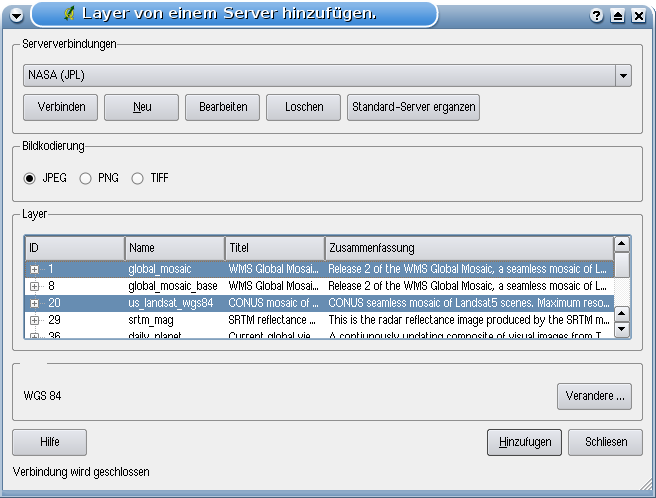
\includegraphics[clip=true,width=0.6\textwidth]{connection_wms}
  \end{center}
\end{figure}

\minisec{Codificaci\'on de imagen}

La secci\'on  \tab{Codificaci\'on de imagen} lista los formatos que son soportados por ambos cliente y servidor.
Elija uno dependiendo de sus requerimientos de exactitud de imagen.

\begin{Tip}[ht]\caption{\textsc{Codificación de la imagen}}
\qgistip{Típicamente encontrará que un servidor WMS le ofrece la elección  de las codificaciones de imágenes JPEG o PNG.  JPEG formato de compresión con pérdida, donde PNG reproduce fielmente los datos raster crudos.

Use JPEG si espera que los datos WMS sean fotográficos en naturaleza y/o no le preocupa pérdida en la  calidad de la fotografía. Esta disyuntiva típicamente reduce 5 veces los requerimientos de tranferencia comparado a PNG.

Use PNG si quiere representaciones precisas de los datos originales, y no le preocupa el incremento de requerimientos en la transmisión de datos.
\index{WMS!image encoding}
}
\end{Tip}

\minisec{Capas} \label{ogc-wms-layers}

La sección \tab{capas} lista las capas disponibles en el servidor WMS seleccionado. Puede notar que algunas capas son expandibles, esto significa que la capa puede ser visualizada con una elección de estilos de imagen.

Puede seleccionar múltiples capas al mismo tiempo, pero solo un estilo de imagen por capa.
Cuando múltiples capas son seleccionadas, serán combinadas en el servidor WMS y transmitido a QGIS en una sola ida.

\begin{Tip}[ht]\caption{\textsc{Ordenamiento de capas WMS}}
\qgistip{En esta versión de QGIS, las capas WMS mostradas por un servidor son sobrepuestas en el orden listado en la sección de capas, de arriba hacia abajo de la lista. Si desea sobreponer capas en el orden opuesto, entonces puede seleccionar \toolbtntwo{mActionAddWmsLayer}{Añadir capa WMS} una segunda vez, elija el mismo servidor nuevamente, y seleccione el segundo grupo de capas que desee sobreponer al primer grupo.

\index{WMS!remote server!layer ordering}
}
\end{Tip}

\minisec{Transparencia}\label{ogc-wms-transparency}

Es esta versión de QGIS, la configuración de transparencia está codificado para estar siempre activa, donde esté disponible.

\begin{Tip}[ht]\caption{\textsc{Transparencia de capas WMS}}
\qgistip{La disponibilidad de transparencia en imágenes WMS depende de la codificación de imagen utilizada:  PNG y GIF suportan transparencia, mientras que JPEG no lo soporta.
\index{WMS!layer transparency}
}
\end{Tip}

\minisec{Sistema de referencia de coordenadas}
\index{WMS!CRS}
\index{WMS!coordinate reference system}
\index{OGC!CRS}
\index{OGC!coordinate reference system}
\index{Projections!WMS}
\index{Projections!CRS}
\index{Projections!coordinate reference system}
\index{CRS}
\index{coordinate reference system}
\index{SRS}
\index{Projections!SRS}

Un sistema de referencia de coordenadas (SRC) es la terminología para una proyección de QGis.

Cada capas WMS puede ser presentada en múltiples SRCs, dependiendo de la capacidad del servidor WMS.  Puede notar los cambios en \textsl{x} 
\textsl{Sistema de Referencia de Coordenadas (x disponibles)} en el encabezado cuando selecciona o deselecciona capas desde la sección \tab{Capa}.

Para elegir un SRC, selecione \button{Cambiar...} y aparecerá una ventana similar a la de la figura \ref{fig:projections} en la sección \ref{label_projstart}.
La diferencia principal con la versión WMS de la pantalla es que solo esos SRCs soportados por el servidor WMS serán mostrados.


\begin{Tip}[ht]\caption{\textsc{Proyecciones WMS}}
\qgistip{Para mejores resultados, haga la capa WMS la primer capa que que agrega a su proyecto. Esto permitirá que la proyección del proyecto herede el SRC usado para mostrar la capa WMS.

La proyección al vuelo (On-the-fly)(vea la sección \ref{sec:projection-specifying}) puede ser usada para acomodar cualquier capa vectorial subsecuente a la proyección del proyecto.

En esta versión de QGIS, si agrega despues una capa WMS, y le da un SRC diferente a la proyección actual del proyecto, puede ocurrir resultados impredecibles.
}
\end{Tip}

% 
% server-search tab.
%
\subsubsection{Búsqueda de servidores}
\label{sec:serversearch}
\index{WMS!serversearch}
\index{WMS!search}
\index{OGC!search}

Dentro de QGIS 1.1.X puede buscar servidores WMS. 
La figura \ref{fig:searchtab} muestra la apenas creada pestaña \tab{buscar} con el diálogo \dialog{Añadir capa(s) de un servidor}.

\begin{figure}[ht]
  \begin{center}
  	\caption{Diálogo para búsquedas de servidores WMS despues de algunas palabras clave \nixcaption}\label{fig:searchtab}
	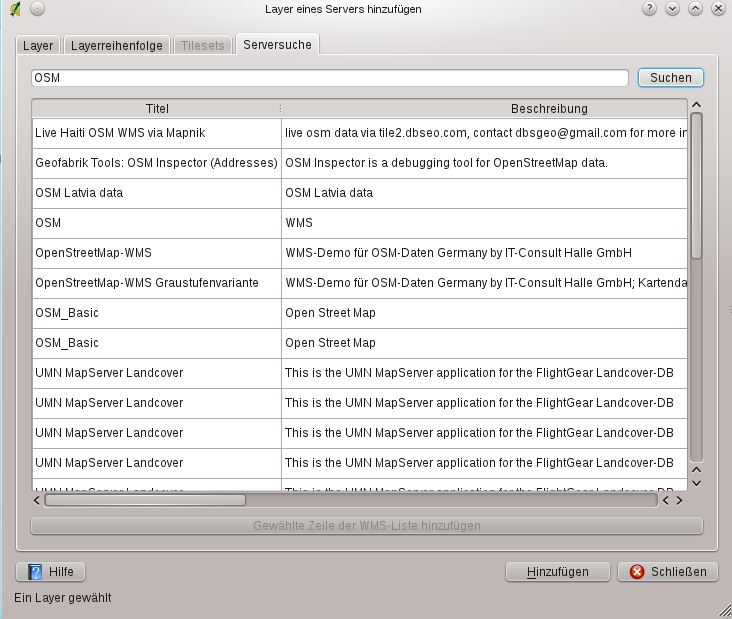
\includegraphics[clip=true,width=0.6\textwidth]{wms_server-search}
  \end{center}
\end{figure}

Como puede ver es posible capturar una cadena de búsqueda en el campo de texto y presionar el botón \button{buscar}.

Después de una pequeña espera el resultado de la búsqueda será llenado dentro de la pestaña debajo del campo de texto.

Navegue la lista de resultados e inspeccione sus resultados de la búsqueda dentro de la tabla. Para visualizar los resultados, seleccione una entrada en la tabla, presione el botón \button{Añadir fila seleccionada a la lista de servidores WMS} y cambie de regreso a la pestaña \tab{servidor}.

QGIS ha actualizado automáticamente la lista de servidores y resultado de búsqueda seleccionado ya está activo en la lista de servidores WMS guardados.

Solo necesita hacer una petición de la lista de capas haciendo clic en el botón \button{conectar}.

Esta opción es muy práctico cuando desea buscar mapas por palabras claves específicas.

Básicamente esta opción es un frontend para la API de
\url{http://geopole.org}.

\subsubsection{Usando la herramienta de identificación}\label{sec:ogc-wms-identify}
\index{WMS!identify}
\index{identify!WMS}
\index{WMS!GetFeatureInfo}

Una vez que ha agregado un servidor WMS, y si cualquier capa del servidor WMS  
acepta búsquedas, entonces puede usar la herramienta \toolbtntwo{mActionIdentify}{Identificar objetos espaciales} para seleccionar un pixel en el canvas del mapa.
Un consulta es hecha al servidor WMS para cada selección realizada.

Los resultados de la consulta  son regresados en texto plano.
el formateo de este texto es dependiente del servidor WMS usado.

\subsubsection{Visualizando propiedades}\label{sec:ogc-wms-properties}\index{WMS!properties}
\index{rasters!properties}

Una vez que ha agregado un servidor WMS, puede visualizar sus propiedades haciendo clic derecho sobre el en la leyenda, y seleccionando \button{Propiedades}.


\minisec{Pestaña metadatos}\label{sec:ogc-wms-properties-metadata}
\index{rasters!metadata}
\index{WMS!metadata}
\index{WMS!capabilites}

La pestaña \tab{metadatos} muestra una gran cantidad de información acerca del servidor WMS, colectado generalmente del resultado de la sentencia Capabilities del servidor.

Muchas definiciones pueden ser recogidas leyendo los estándares WMS
\cite{OGCWMS010101web}, \cite{OGCWMS010300web}, pero aquí hay algunas definiciones prácticas:

\begin{itemize}
\item \textbf{Propiedades del servidor}

\begin{itemize}
\item \textbf{Versión WMS}      - La versión WMS soportada por el servidor.

\item \textbf{Formatos de imagen}    - La lista de tipos MIME con los que el servidor puede responder cuando dibuja el mapa.  QGIS soporta cualquier formato con que haya sido compilado la librería Qt subyacente, las cuales son al menos \texttt{image/png} y \texttt{image/jpeg}.

\item \textbf{Formatos de indetificación} - La lista de los tipos MIME con los que el servidor puede responder cuando usa la herramienta de identificación.  Actualmente QGIS soporta el tipo  \texttt{text-plain}.

\end{itemize}

\item \textbf{Propiedades de la capa}

\begin{itemize}
\item \textbf{Seleccionado}         - Si esta capa fue seleccionada o no cuando su servidor fue añadido a este proyecto.

\item \textbf{Visible}          - Si esta capa fue seleccionada como visible o no en la leyenda.  (No es usado todavía en esta versión de QGIS.)

\item \textbf{Puede identificar}     - Si esta capa regresará o no resultados cuando la herramienta de identificar sea usada en ella.

\item \textbf{Puede ser transparente} - Si esta capa puede ser presentada con transparencia  o no. Esta versión de QGIS usará siempre transparencia si esto es \textsl{Si} y la codificación de la imagen soporta transparencia.

% BM: doesn't seem to work?
%                                    (see Section
%                                    \ref{ogc-wms-transparency}
%                                    ).
                                    .

\item \textbf{Puede acercarse}      - Si se le puede hacer zoom a esta capa por el servidor o no. Esta versión de QGIS asume que todos los servidores tiene esto establecido a \textsl{Si}. Capas deficientes pueden ser presentadas extrañamente.

\item \textbf{Conteo de cascada}    - Los servidores WMS pueden actuar como un proxy para otros servidores WMS para obtener datos raster para una capa. Esta entrada muestra cuantas veces la petición para esta capa es transmitido a otros servidores WMS para un resultado.

\item \textbf{Ancho fijo}, \textbf{Altura fija}
                                - Si esta capa tiene dimensiones fijas en la fuente. Esta versión de QGIS asume todas las capas WMS tiene esto establecido a nada. Capas deficientes pueden ser presentadas extrañamente.

\item \textbf{Caja WGS 84} - La caja de la capa, en coordenadas WGS 84. Algunos servidores no establecen esto correctamente (ej. son usadas coordenadas UTM). Si este es el caso, entonces la vista inicial de esta capa puede ser presentada con un apariencia de un gran alejamiento por QGIS. El webmaster del servidor WMS debe ser informado de este error, el cual deber ser conocido por ellos como el elemento xml del WMS                                     \texttt{LatLonBoundingBox},                                      \texttt{EX\_GeographicBoundingBox} o el SRC:84 \texttt{BoundingBox}.

\item \textbf{SRC disponible} - Las proyecciones en las que esta capa puede ser presentada por el servidor WMS.  Estos son listados en el formato nativos del WMS.

\item \textbf{Disponible en estilos} - Los estilos de imagen que esta capa puede ser presentada por el servidor WMS.

\end{itemize}

\end{itemize}


\subsubsection{Limitaciones del cliente WMS}\label{sec:ogc-wms-limits}\index{WMS!client!limits}

No toda la funcionalidad de cliente WMS ha sido incluida en esta versión de  QGIS.
Algunas de las excepciones mas notables son:

\minisec{Edición de configuraciones de capa wms}
\index{WMS!layer settings!editing}

Una vez que ha completado el procedimiento \toolbtntwo{mActionAddWmsLayer}{Añadir capa WMS }, no existe la habilidad para cambiar las configuraciones.

Una forma alternativa es borrar la capa WMS completamente y empezar nuevamente.

\minisec{Servidores WMS que requieren autenticación}
\index{WMS!remote server!authentication}
\index{WMS!remote server!basic authentification}

Actualmente son soportados los servicios públicamente disponibles y servidores seguros.

Los servidores WMS seguros pueden ser accesados con autenticación pública. Puede agregar las credenciales (opcionales) cuando agrega un servidor WMS. Vea la sección \ref{sec:ogc-wms-servers} para mas detalles.

\begin{Tip}[ht]\caption{\textsc{Accesando capas OGC seguras}}
\qgistip{Si necesita accesar capas seguras con otros métodos de seguridad diferentes a la autentificación básica, puede usar el InteProxy como un proxy transparente, el cual soporta varios métodos de autenticación.
Mas información puede ser encontrada en el manual InteProxy-manual encontrado en el sitio web \url{http://inteproxy.wald.intevation.org}. \index{WMS!secured layers!}\index{OGC!Authentication}
}
\end{Tip}


\subsection{Cliente WFS}\label{sec:ogc-wfs}

En QGIS, una capa WFS se comporta de forma muy parecidad a cualquier otro capa vectorial. Puede identificar y seleccionar objetos espaciales y ver la tabla de atributos. Una excepción es que la edición no es soportada al momento. Para iniciar el complemento WFS  necesita abrir \mainmenuopt{Complementos} > \dropmenuopttwo{mActionShowPluginManager}{Manejador de complementos...}, 
activar la caja de selección \checkbox{Complemento WFS} y hacer clic en \button{OK}. 

Un nuevo ícono aparece \toolbtntwo{mIconAddWfsLayer}{Añadir capas WFS} despues del ícono WMS. Haga clic en el para abrir el diálogo. En general agregar una capa WFS es muy similar al procedimientos usado con WMS. La diferencia es que no hay servidores predeterminados, de manera que tenemos que agregar los nuestros.

\subsubsection{Cargando una capas WFS}

Como ejemplo usamos el servidor de DM Solutions WFS server y mostramos una capa. La URL es:
\begin{verbatim}
http://www2.dmsolutions.ca/cgi-bin/mswfs_gmap?VERSION=1.0.0&SERVICE=
wfs&REQUEST=GetCapabilities
\end{verbatim}

\begin{enumerate}
  \item Asegúrese que el complemento WFS está cargado; si no, abra el manejador de plugins y cárguelo
  \item Haga clic en la herramienta 
  \toolbtntwo{mIconAddWfsLayer}{Añadir capa WFS} 
  de la barra de herramientas de complementos
  \item Haga clic en  \button{Nuevo} 
  \item Escriba \inputtext{Nombre}{DM Solutions} como el nombre
  \item Escriba la URL (ve la página previa)
  \item Haga click en \button{OK} 
  \item Elija \selectstring{Conexiones de servidor}{DM Solutions} de la lista desplegable
  \item Haga clic en \button{Connectar} 
  \item Espera que la lista de capas sea llenada
  \item Haga clic en la capa \clicklistitem{Canadian Land}
  \item Haga clic en \button{Añadir} para agregar la capa al mapa
  \item Espere pacientemente a que los objetos espaciales.
\end{enumerate}

Note that the WFS-plugin also recognizes the proxy-settings you have set
in your preferences.

\begin{figure}[ht]
  \begin{center}
  	\caption{Añadiendo una capa WFS \nixcaption}\label{fig:wfs_dmsolutions}
	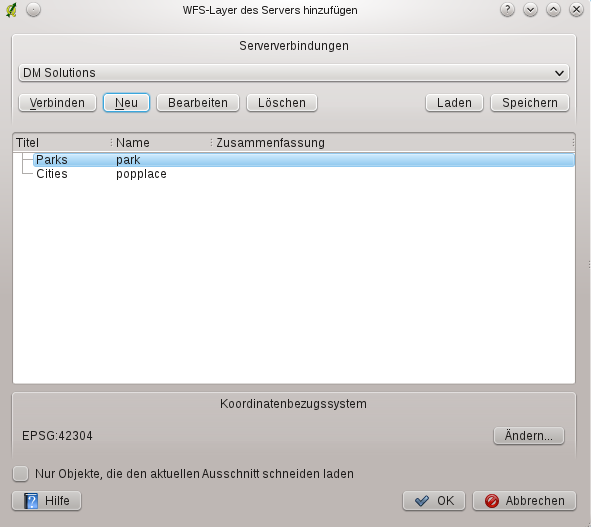
\includegraphics[clip=true,width=0.6\textwidth]{connection_wfs}
  \end{center}
\end{figure}

Notará que el progreso de la bajada  es visualizado en la parte inferior izquierda de la ventana principal de QGIS. 
Una vez que la capa es cargada, puede identificar y seleccionar una provincia o dos y ver la tabla de atributos.

Recuerde que es plugin trabaja mejor con servidores WFS de UMN MapServer. Puede aun ser, que experimente comportamiento aleatorio y falle. Puede esperar mejoras en versiones futuras del complemento.

Esto significa que solo WFS 1.0.0 es soportado. A este punto ha habido muchas pruebas contra versiones WFS implementados en otros servidores WFS. Si encuentra problemas con algún otro servidor WFS, por favor no dude en contactar al equipo de desarrollo. Por favor remítase a la sección 
\ref{label_helpsupport} para mayor información acerca de las listas de correo.

\begin{Tip}[ht]\caption{\textsc{Encontrando servidores WFS}}
\qgistip{Puede encontrar servidores WFS adicionales usando google o su motor de búsquedas favorito. Hay un número de listas con URLs públicas, algunas de ellas con mantenimiento y otras no.
\index{WFS!remote server!}
}
\end{Tip} 

\begin{Tip}[ht]\caption{\textsc{Accesando servidores WFS seguros}}
\qgistip{
Dentro del diálogo \dialog{Crear una nueva conexión WFS} accidentalmente descrito QGIS aun no soporta conexiones WFS autenticadas. Dentro de una de las proximas liberaciones esperamos también soportar servidores WFS autentticados. Por lo pronto puede usar InteProxy
(\url{http://inteproxy.wald.intevation.org}) para accesar a servidores WFS autenticados.
\index{WFS!authenticate remote server!}
\index{WFS!secured WFS server!}
}
\end{Tip} 

